\documentclass[xcolor=dvipsnames]{beamer}
\mode<presentation> {

\usecolortheme{default}
%\setbeamercovered{transparent}

\definecolor{carolina}{HTML}{82CAFA}
%\definecolor{carolina}{HTML}{3BB9FF}
%\definecolor{gray}{HTML}{B6B6B4}
%\definecolor{dark}{HTML}{151B54}

\usetheme{Madrid}
\setbeamercolor{structure}{fg=carolina}
\setbeamercolor{block title}{bg=carolina}
\setbeamercolor{block title example}{bg=carolina}

%Uncomment the following if you prefer for the font color on carolina blue background to be black.
%\setbeamercolor{block title}{fg=black,bg=carolina}
%\setbeamercolor{frametitle}{fg=black}
%\setbeamercolor{title}{fg=black}

\setbeamertemplate{caption}[numbered]
\setbeamertemplate{enumerate items}[circle]
\setbeamertemplate{itemize items}[circle]
\setbeamertemplate{section in toc}[circle]
\setcounter{tocdepth}{1} 
\setbeamercolor{section in toc}{fg=black}

\usefonttheme[onlymath]{serif}

%\setbeamertemplate{footline} % To remove the footer line in all slides uncomment this line
%\setbeamertemplate{footline}[page number] 

% To replace the footer line in all slides with a simple slide count uncomment this line
%\setbeamertemplate{navigation symbols}{}

% To remove the navigation symbols from the bottom of all slides uncomment this line
}

%some commonly used packages
\usepackage{graphics}
\usepackage{graphicx}
\usepackage{tikz}
\usepackage{fancyvrb}
\usepackage{comment}
\usepackage{amsmath}
\usepackage{amssymb}
\usepackage{lipsum}
\usepackage{subcaption}
\usepackage{caption}
\usepackage{comment}
\usepackage{multi row}
\usepackage{copyrightbox}
\usepackage{pdflscape}
\usepackage{url}
\usepackage{hyperref}

\newcommand{\overbar}[1]{\mkern 1.5mu\overline{\mkern-1.5mu#1\mkern-1.5mu}\mkern 1.5mu} %Instead of \bar or \overline, use \overbar for proper length and thickness bar for sample average. 

%Edit the following lump of code to customize with your name, title, and date
\title[Data Management]{Wrangling Your Data}
\author[Kevin Donovan]{Kevin Donovan}
\institute[UNC and IBIS]{UNC-Chapel Hill and IBIS Network}
\date[11/12/2020]{11/12/2020}

\newcounter{saveenumi}
\newcommand{\seti}{\setcounter{saveenumi}{\value{enumi}}}
\newcommand{\conti}{\setcounter{enumi}{\value{saveenumi}}}

\resetcounteronoverlays{saveenumi}

\begin{document}

\begin{frame}
	\titlepage
\end{frame}

\section{Wrangling Your Data}
\begin{frame}
\frametitle{\insertsectionhead}
\textbf{Data in given form often not suitable for analysis}
\begin{itemize}
\item Create new variables
\item Rearrange variable order
\item Rearrange row order
\item Remove observations
\begin{figure}
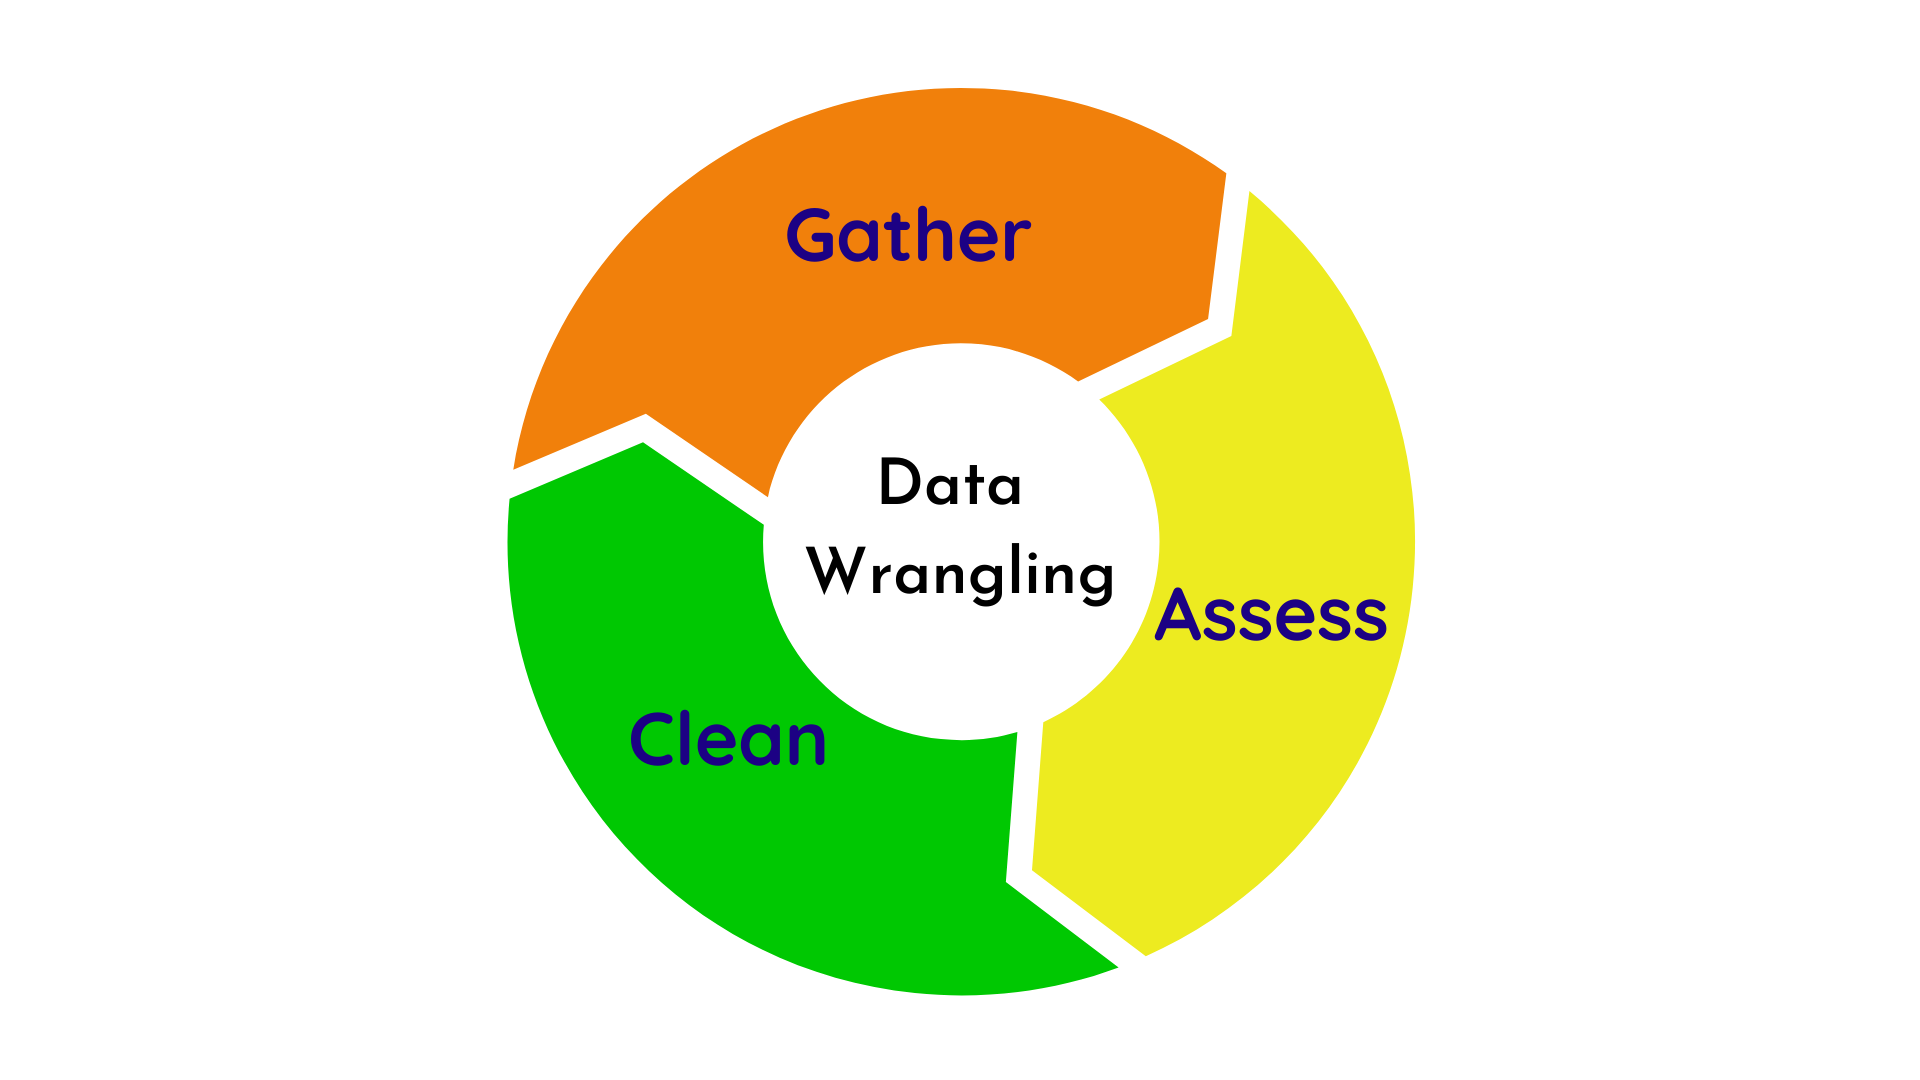
\includegraphics[scale=0.1]{images/data_wrangling.png}
\end{figure}
\end{itemize}
\end{frame}

\begin{frame}
\frametitle{\insertsectionhead}
\textbf{Benefits of using R}
\begin{itemize}
\item Can edit temporary versions of data
\item All in code; transparent/reproducible
\item Easily save output in various formats
\item Very powerful tools
\end{itemize}
\end{frame}

\begin{frame}
\frametitle{\insertsectionhead}
\textbf{R Data Structure}\\
Standard Format: \textbf{Data Frame}
\begin{figure}
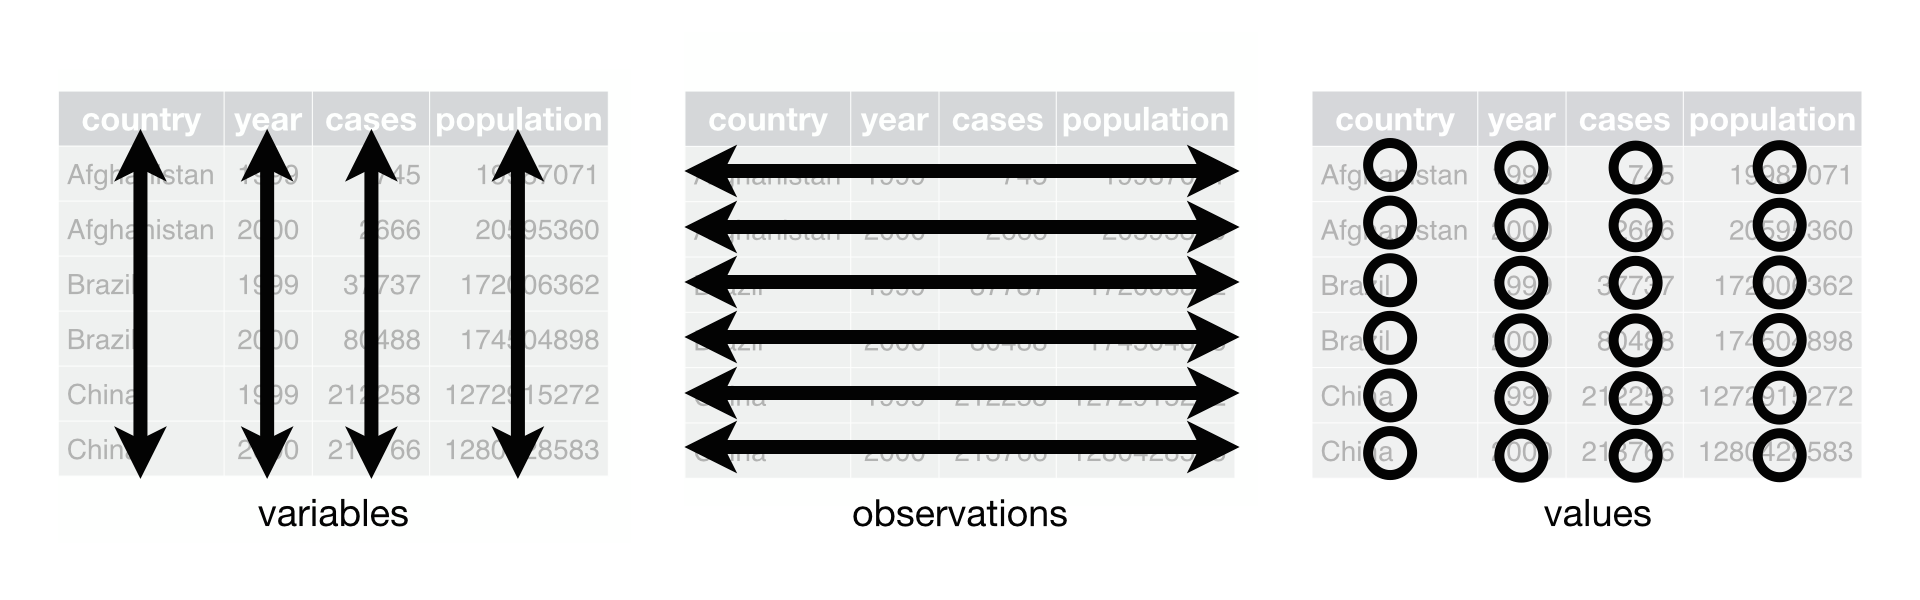
\includegraphics[scale=0.18]{images/tidy_data.png}
\end{figure}
Data in \textbf{Tidy} form
\end{frame}

\begin{frame}
\frametitle{\insertsectionhead}
\textbf{Methods in R}\\
\begin{itemize}
\item Base R (built-in functions)
\item Tidyverse packages
\begin{figure}
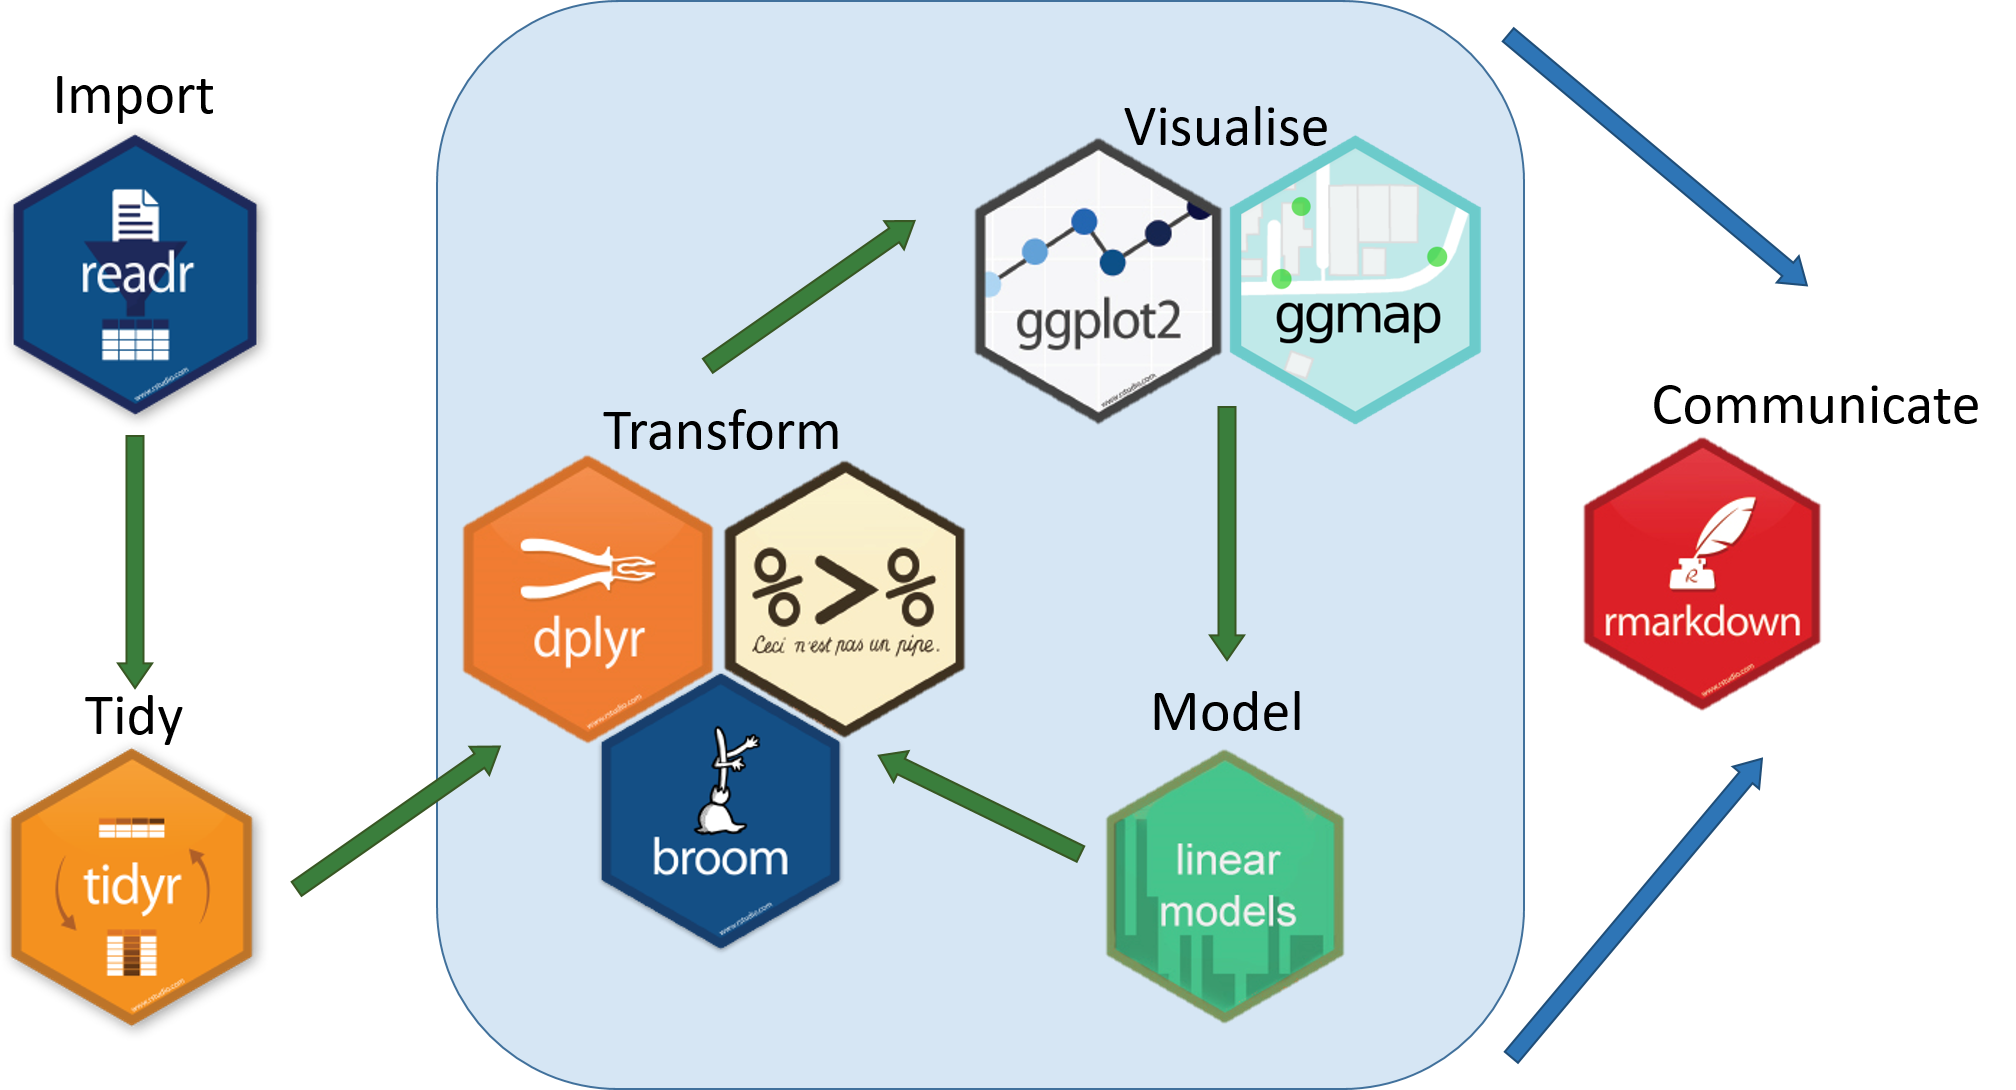
\includegraphics[scale=0.3]{images/tidyverse.png}
\end{figure}
\end{itemize}
\end{frame}

\section{Song of the Session}
\begin{frame}
\frametitle{\insertsectionhead}

\end{frame}

\end{document}

